\documentclass[main]{subfiles}
\begin{document}

%@@@@@@@@@@@@@@@@@@@@@@@@@@@@@@
% Main Topics: Perceptron Learning Algorithm 06.12.2018
% Lecturer: Matthew Cook
% author: Vanessa Leite - base document from benelot/eth-intro-to-neuroinformatics-summary

\section{Perceptron}

\subsection{Threshold function}

\begin{figure}[H]
	\centering
	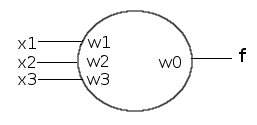
\includegraphics[width=0.3\textwidth]{linear-threshold.png}
\end{figure}

\[ f(\vec{x}) = \theta(\vec{w} \times \vec{x} + w_0) \]
\[ f(x_1, x_2, x_3) = \theta(w_1 \times x_1 + w_2 \times x_2 + w_3 \times x_3 + w_0) \]

\[
    \theta(x)= 
\begin{cases}
     0, & \text{if } x < 0\\
     1, & \text{if } x \geq 0
\end{cases}
\]

\subsection{Converting real weights to integer}
Any unit can be converted into one with integer weights.

\begin{figure}[H]
	\centering
	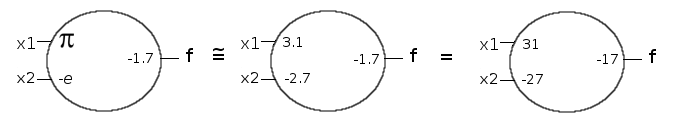
\includegraphics[width=0.8\textwidth]{converting-units-integer.png}
	\caption{Converting real weights to integer}
	\label{fig:converting}
\end{figure}

Figure~\ref{fig:converting} shows the approach to convert real weights to integer. The approximation (images left and center) can be problematic if $x$ in $\theta(x)$ is equal to zero (in the real setup), because it can be shifted in the approximation.
In the second step (images center and right) there is no problem. By multiplying the weights per a factor of 10, we do not change the value of $x$ in $\theta(x)$.

One way to solve the above problem (approximation) is to shift the bias term a bit.

\begin{enumerate}
\item Find the largest possible negative sum (closest to zero)
\item Adjust bias (increase) if necessary so no sum is zero
\item Replace weights with rational approximations more precise than sum closest to zero
\item Scale up weights to be integers
\end{enumerate}

In the first two steps, we avoid have a sum of zero. On the last two, we transform the weights to integer.

So far, the difference of this unit and a real neuron is that neurons can adjust their own weight (learning) and these units are behaving as gates.

\subsection{Perceptron Learning Algorithm}

\begin{table}[H]
\begin{tabular}{cc|c}
x1 & x2 & f \\ 
\hline
0  & 0  & 1 \\
0  & 1  & 0 \\
1  & 0  & 1 \\
1  & 1  & 1 \\ 
\end{tabular}
\end{table}

Can we set $w_0, w_1, w_2$ so that this unit computes the above $f$?
We start with random weights, let's say all zero. With this weights, doesn't matter the values of $x_1$ and $x_2$, the result will always be 1. And for the second case ($x_1 = 0, x_2 = 1, f = 0$) we produce a wrong output.

So, we reduce $w_0$ and $w_2$ because they contribute to the sum ($0 \times w_1 + 1 \times w_2 + w_0$). We reduce the weights if the sum should go down and we increase the weights if the sum should go up. We iterate this step until convergence.

We can consider the bias as a weight with input value always one ($x_0 = 1$), thus, we can write:

\[ f(\vec{x}) = \theta(\vec{w} \times \vec{x} + w_0) = \theta(\vec{w} \times \vec{x}) \]

\paragraph{Recall} $\vec{w} \times \vec{x} = |\vec{w}| \times |\vec{x}| \times \cos \alpha$.  So, if $\alpha < 90\deg$, $\vec{w} \times \vec{x}$ is greather than zero and if $\alpha > 90\deg$, $\vec{w} \times \vec{x} < 0$.

This way, we compute a similarity between the weight vector and the input vector.

The weights of the Perceptron can be seen as the components of a normal vector to the hyperplane that separates the classes ($1$ and $0$). In  fact, the  length of the normal vector doesnt matter, we are looking for its direction.

\paragraph{Convergence}
Suppose there is a solution $\vec{w}^*$, i.e., the data is linearly separable.
Pick any solution $\vec{w}$, for instance, starting with all weights as zero, if this solution already satisfies our conditions, we are done. Otherwise, we pick an arbitrary missclassified point and update $\vec{w}$. Each step makes progress in the $\vec{w}^*$ direction, because additions to $\vec{w}$ are always $\leq 90\deg$. The magnitude of $\vec{w}^* \times \vec{w}$ increases linearly. Since $\vec{w}^*$ doesn't change, there is a maximum growth from $\vec{w}$ to achieve the solution.
By contradiction in the limit of infinite steps, we can say that the algorithm converges, i.e., if there is a solution and it takes infinite steps to achieve it, this is a contradiction.

\paragraph{Algorithm}
\begin{itemize}[noitemsep,nolistsep]
	\item Choose random initial weights.
	\item Calculate output for given input.
	\item If the output is not the expected value, then $e=d-c$, where $d$ is the desired output and $c$ the current output.
	\item Change the weight of inputs and bias by $\Delta w_i=e\cdot\alpha\cdot x_i$. For the bias, always use $x=1$.
\end{itemize}

\end{document}
